% \chapter{Đánh giá}

\section{Đánh giá chất lượng đầu ra của lộ trình học đề xuất bởi LLM}

\subsection{Phương án đánh giá}
Trong bối cảnh đánh giá hệ thống sinh lộ trình học tập, có hai hướng tiếp cận để đánh giá \cite{zhang2020new}:
\begin{itemize}
    \item \textbf{Online evaluation} là phương pháp sử dụng phản hồi thực tế từ người dùng hoặc chuyên gia để đánh giá chất lượng đầu ra. Phương pháp này có độ tin cậy cao và phản ánh đúng nhu cầu thực tế, tuy nhiên yêu cầu thời gian, chi phí lớn và khó mở rộng trong giai đoạn phát triển ban đầu.
    \item \textbf{Offline evaluation} là phương pháp sử dụng mô hình hoặc thuật toán đánh giá tự động để đánh giá đầu ra mà không cần tương tác với người dùng, về dữ liệu, những dữ liệu cũ quan sát được trong quá khứ có thể được sử dụng cho Offline evaluation.
\end{itemize}
Trong phần đánh giá này, nhóm lựa chọn phương pháp \textbf{offline evaluation kết hợp với GEval} – một framework đánh giá tự động sử dụng mô hình ngôn ngữ lớn (LLM) làm giám khảo (LLM-as-a-Judge)\cite{liu2023gevalnlgevaluationusing}. GEval cung cấp một framework linh hoạt để định nghĩa các tiêu chí đánh giá tuỳ chỉnh, kết hợp với chuỗi suy luận (Chain-of-Thought) để hướng dẫn mô hình đưa ra lập luận có cơ sở. GEval có những điểm phù hợp để được chọn làm metric cho  phần đánh giá này vì:
\begin{itemize}
    \item Không cần dữ liệu tham chiếu cố định (reference output).
    \item Thực hiện đánh giá nhanh, lặp đi lặp lại và có thể tự động hóa được với nhiều tập dữ liệu khác nhau.
    \item Dễ mở rộng cho nhiều tiêu chí khác nhau như chất lượng giải thích, tính logic, mức độ phù hợp mục tiêu,...
    \item Có thể sử dụng với nhiều mô hình đánh giá khác nhau như: gpt-4o, gpt-4o-mini, llama-3.2,...
\end{itemize}

\subsection{Xây dựng các metrics}
Dựa trên metric GEval được đề cập ở trên, các metric sau được lựa chọn để đánh giá sơ bộ đầu ra của hệ thống:
\begin{itemize}
    \item \textbf{Goal Alignment (Goal)}: Lộ trình có bám sát mục tiêu học tập không?
    \item \textbf{Explanation Quality (Expl.)}: Chất lượng và độ rõ ràng của giải thích lý do trong từng bài học được đề xuất.
    \item \textbf{Ordering Logic (Order)}: Trình tự các bài học có hợp lý và phát triển kiến thức tuyến tính không?
    \item \textbf{Module Appropriateness (Mod. App.)}: Các module có phù hợp với nội dung bài học và mục tiêu không?
\end{itemize}

Metric GEval được sử dụng làm nền tảng để tự động hóa quá trình đánh giá, cụ thể:
\begin{itemize}
    \item Xây dựng tiêu chí đánh giá cho từng metrics, tương tự như việc xây dựng một rubrics để chấm điểm và các tiêu chí này phải càng cụ thể, giống như con người thực hiện việc đánh giá cũng cần rubrics.
    \item Model đánh giá (evaluator) được yêu cầu cho điểm (score) và giải thích (reasoning).
\end{itemize}
Chi tiết về các metrics được định nghĩa cho phần đánh giá, người đọc có thể xem chi tiết ở đoạn code sau: \href{https://github.com/dpnam2112/codemate-backend/blob/main/tests/metrics.py}{Github}\footnote{Định nghĩa các metrics: \url{https://github.com/dpnam2112/codemate-backend/blob/main/tests/metrics.py}}.

\subsection{Thiết kế quy trình đánh giá}
Do hạn chế về tài nguyên cũng như một số ràng buộc từ các nhà cung cấp dịch vụ để sử dụng mô hình của OpenAI, Google,... nên hiện tại, nhóm chỉ có thể triển khai việc đánh giá với phương pháp này ở mức cơ bản và về mặt ý tưởng:
\begin{itemize}
    \item Mô hình sinh lộ trình: \emph{Gemini 2.0 Flash}.
    \item Các mô hình đánh giá: \emph{gpt-4o-mini}, \emph{gpt-4.1-nano}, \emph{llama-3.3-70B}. Ta cần sử dụng các mô hình không cùng họ với mô hình sinh lộ trình do phương án LLM-as-a-judge có một nhược điểm: Nếu LLM được sử dụng như là người đánh giá cùng họ/có đặc tính tương đồng với mô hình được sử dụng để sinh ra output, thì việc thiên vị trong đánh giá có thể xảy ra do vấn đề \emph{Preference leakage}\cite{li2025preferenceleakagecontaminationproblem}.
    \item Dữ liệu đầu vào: Mục tiêu học tập cụ thể của học sinh cho từng khóa học. Người đọc có thể tham khảo thêm về dữ liệu được sử dụng để đánh giá ở đường link sau: \href{https://github.com/dpnam2112/codemate-backend/blob/main/evaluation/data/learning_path/learning_paths_20250429-1307.json}{Github}\footnote{Dữ liệu bài tập code và lời giải: \url{https://github.com/dpnam2112/codemate-backend/blob/main/evaluation/data/learning_path/learning_paths_20250429-1307.json}}.
    \item Output: File CSV lưu kết quả điểm số và giải thích cho từng metric.
    \item Khóa học được sử dụng để thực hiện đánh giá:
    \begin{itemize}
        \item Cấu trúc dữ liệu và giải thuật của Đại học Bách khoa thành phố Hồ Chí Minh.
        \item Nhập môn Khoa học máy tính và lập trình bằng Python của MIT (MIT 6.0001)
    \end{itemize}
\end{itemize}

\subsection{Kết quả đánh giá và nhận xét}

Sau khi thực thi code để đánh giá, ta thu được các kết quả sau:

Kết quả đánh giá (file csv): \href{https://github.com/dpnam2112/codemate-backend/blob/main/evaluation/data/lp_csv/lp_csv_gpt_and_llama.csv}{Github}\footnote{Dữ liệu kết quả đánh giá learning path: \url{https://github.com/dpnam2112/codemate-backend/blob/main/evaluation/data/lp_csv/lp_csv_gpt_and_llama.csv}}

\begin{table}[h!]
\centering
\caption{Điểm trung bình theo từng tiêu chí đánh giá: Goal, Explanation Quality, Module Appropriateness, và Ordering Logic}
\begin{tabular}{lcccc}
\toprule
\textbf{Model} & \textbf{Expl.} & \textbf{Goal} & \textbf{Mod. App.} & \textbf{Order} \\
\midrule
gpt-4.1-nano & 0.883 & 0.867 & 0.900 & 0.817 \\
gpt-4o-mini  & 0.917 & 0.883 & 0.950 & 0.767 \\
LLaMA-3.1-70B & 0.945 & 0.964 & 0.945 & 0.891 \\
\bottomrule
\end{tabular}

\label{tab:avg_scores_abbr}
\end{table}

\begin{figure}[H]
\centering
    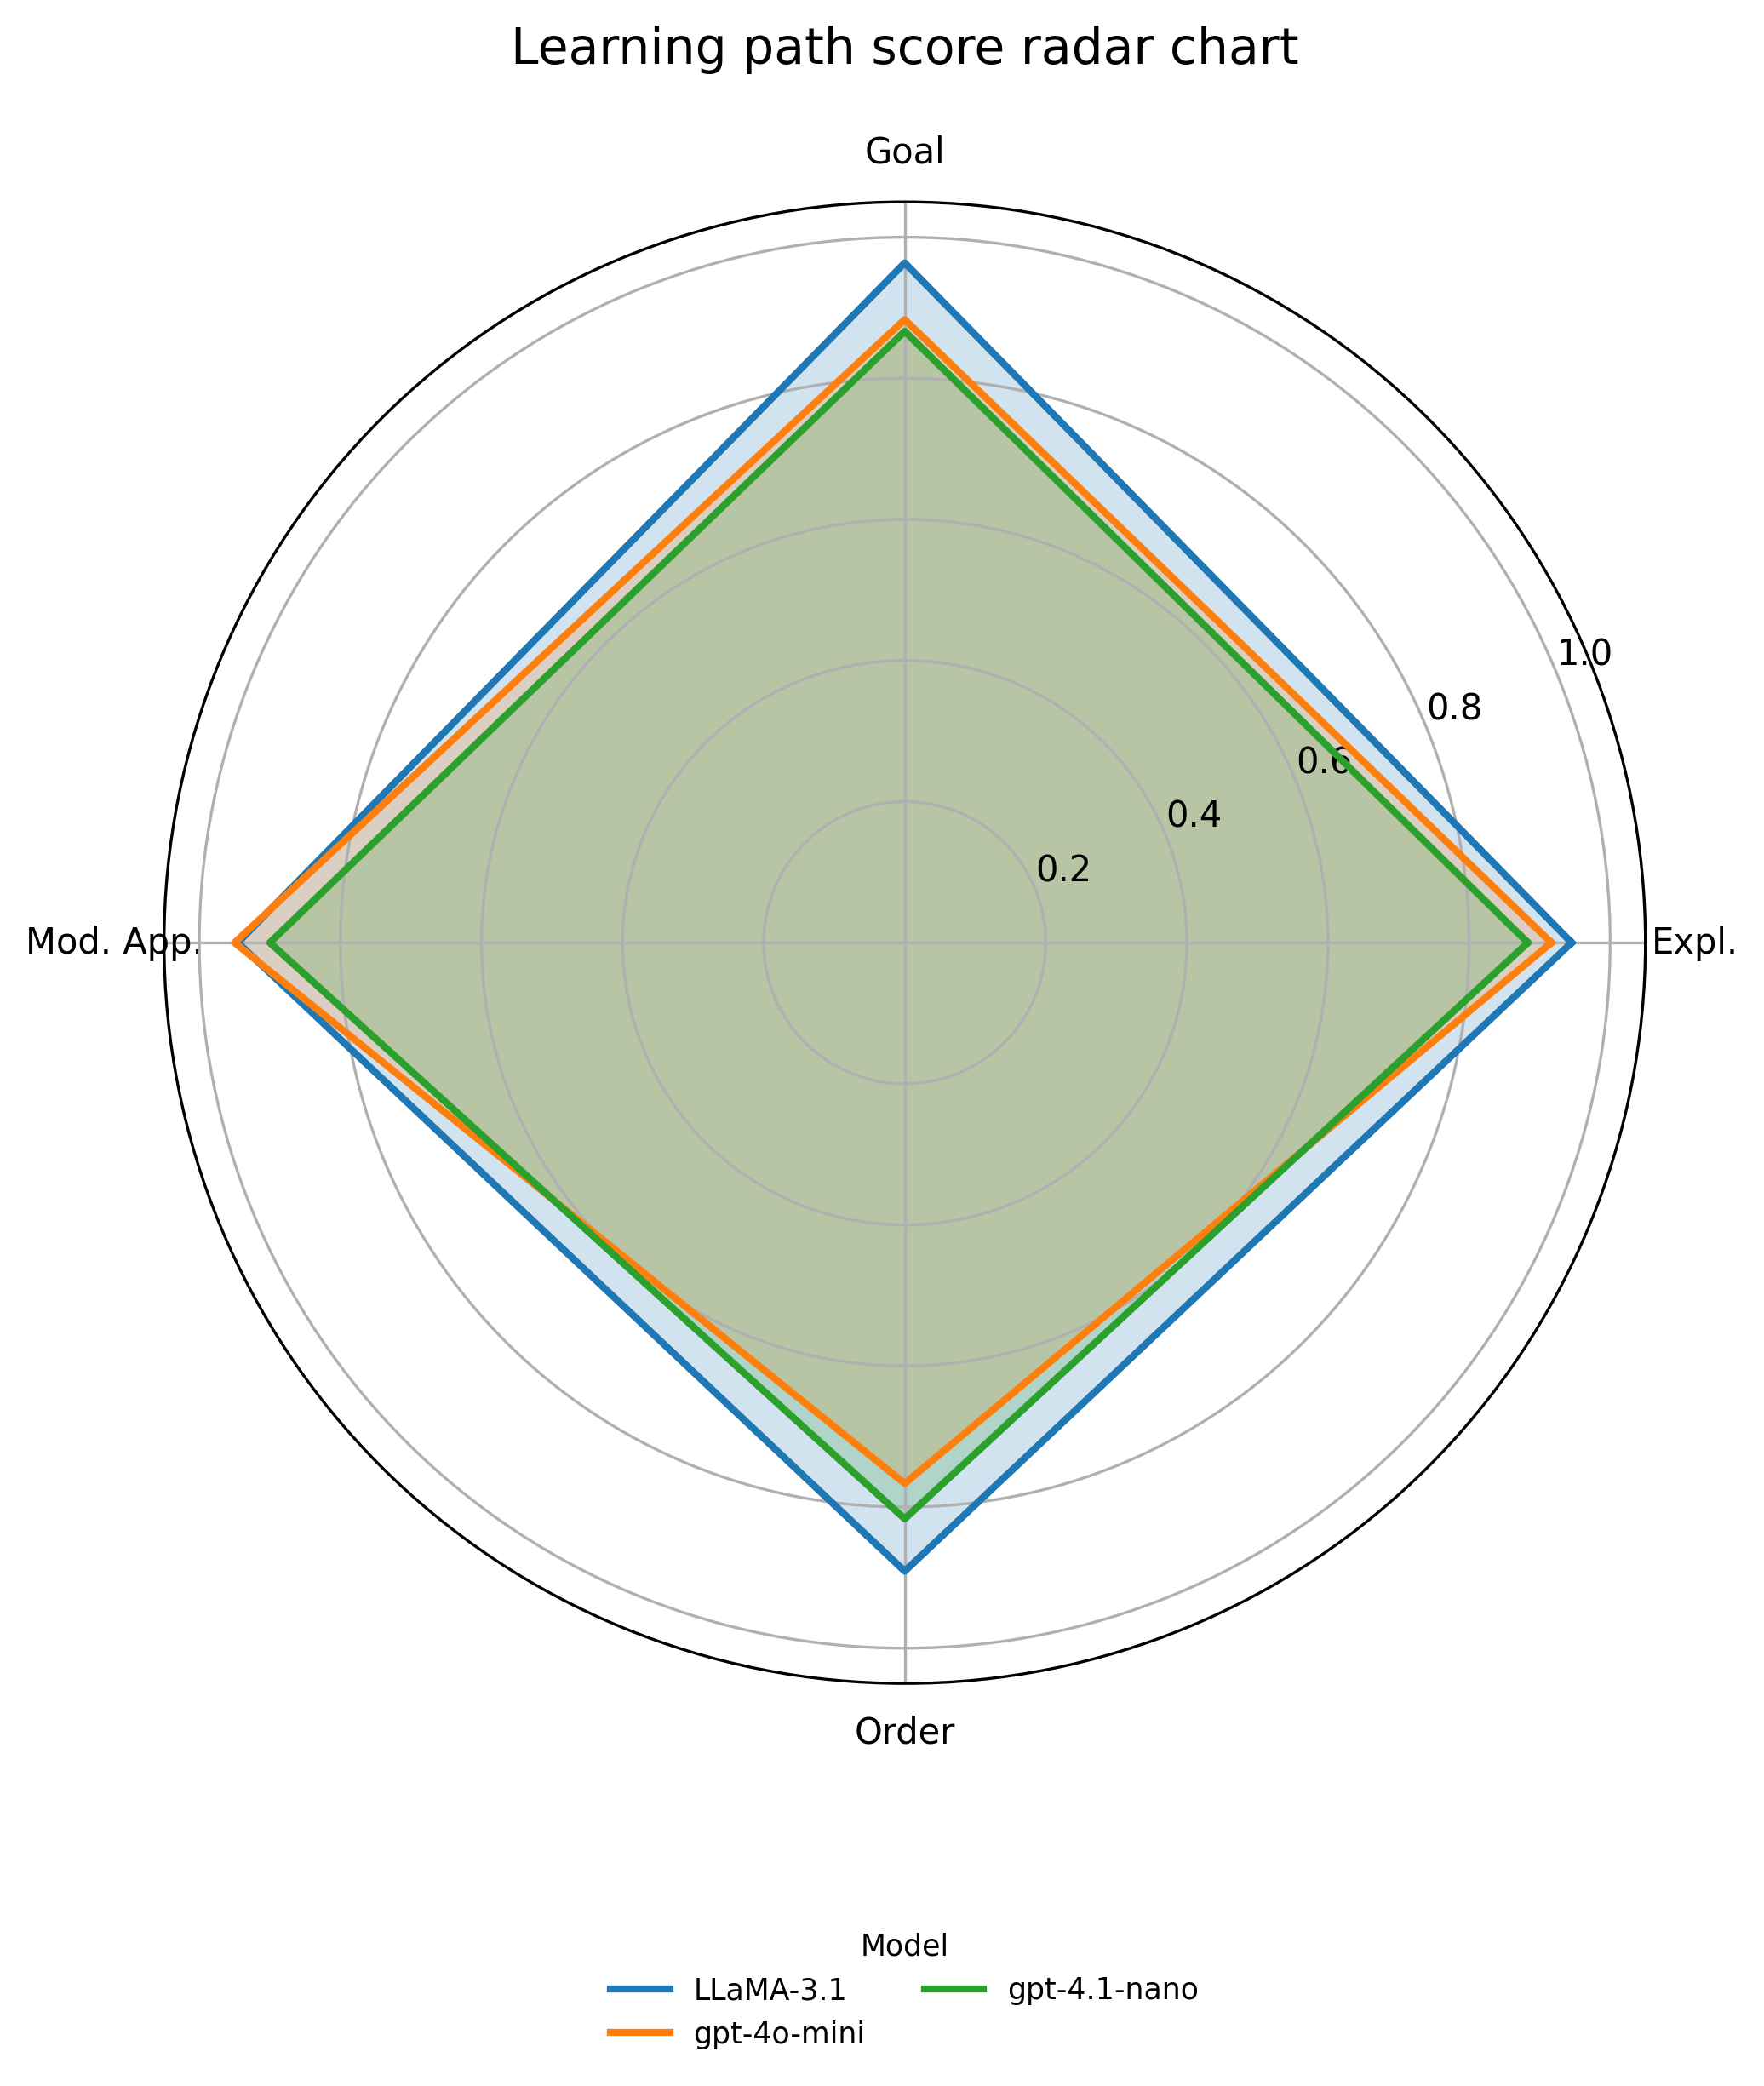
\includegraphics[width=0.6\textwidth]{images/lp_eval_radar_chart.png}
    \caption{Radar chart tổng hợp kết quả đánh giá lộ trình học đề xuất khi chạy đánh giá LLM-as-a-judge ứng với từng model}
\end{figure}

Dựa vào kết quả có được, sau đây là một số nhận xét sơ bộ:
\begin{itemize}
    \item Tiêu chí \textbf{Explanation Quality} đạt điểm trung bình cao nhất (0.917 theo gpt-4o-mini hay 0.883 theo gpt-4.1-nano), cho thấy phần lớn các bài học trong lộ trình đều có phần giải thích rõ ràng, dễ hiểu và phù hợp với nội dung.

    \item Về tiêu chí \textbf{Module Appropriateness}, hệ thống cũng ghi nhận mức đánh giá tích cực (lên đến 0.95), cho thấy các module học tập được lựa chọn và tạo sinh phù hợp với từng bài học và mục tiêu tổng thể, không bị lệch pha hay dư thừa nội dung.

    \item Tiêu chí \textbf{Goal Alignment} có điểm số ổn định (khoảng 0.88), phản ánh rằng lộ trình học tập nhìn chung bám sát mục tiêu đầu vào mà người học đã đặt ra.

    \item Tuy nhiên, ở tiêu chí \textbf{Ordering Logic}, điểm số trung bình thấp hơn đáng kể (0.767 theo gpt-4o-mini, 0.817 theo gpt-4.1-nano). Điều này cho thấy vẫn còn tồn tại một số vấn đề về thứ tự sắp xếp các bài học – ví dụ như thiếu tính tuyến tính, sắp xếp không tối ưu về mặt xây dựng nền tảng kiến thức.
\end{itemize}

\section{Đánh giá testcases được sinh ra bởi tính năng tạo sinh bài tập code}
\subsection{Phương pháp đánh giá}
Trong bối cảnh đánh giá chất lượng test case được sinh tự động bởi LLM nói riêng cũng như chất lượng của một bộ testcases nói chung, có nhiều metrics khác nhau có thể được xem xét, bao gồm:
\begin{itemize}
    \item Tính đa dạng (Diversity) đo mức độ khác biệt giữa các test case trong một bộ dữ liệu.
    \item Độ phủ (Coverage) đo xem test case có bao phủ đủ các nhánh logic, điều kiện biên, hoặc tập input không.
    \item Mutation Score là tỉ lệ mutant (phiên bản lời giải bị chỉnh sửa nhỏ để cố tình tạo lỗi) bị phát hiện bởi test case. Chỉ số này phản ánh khả năng của test case trong việc phân biệt giữa lời giải đúng và lời giải sai — tức là đo mức độ “sắc bén” của test case trong kiểm thử.

\end{itemize}

Tuy nhiên, trong phạm vi đánh giá sơ bộ này, nhóm lựa chọn một metric đơn giản nhưng có giá trị thực tiễn là: \textbf{tỉ lệ test case chạy đúng (pass)} khi thực thi với một lời giải đã được kiểm chứng là chính xác với các lý do như sau:
\begin{itemize}
    \item Đây là bước kiểm tra cơ bản và thiết yếu, nếu test case không chạy được hoặc gây lỗi, các đánh giá khác sẽ không còn ý nghĩa.
    \item Dễ triển khai và so sánh giữa các mô hình sinh test case khác nhau.
    \item Phản ánh gián tiếp khả năng hiểu đề và sinh đầu vào hợp lệ của mô hình.
\end{itemize}

Phép đánh giá được thực hiện bằng cách chạy từng test case trên một lời giải mẫu được xác nhận là đúng, sử dụng môi trường thực thi tự động (Judge0). Các kết quả như “Pass”, “Fail”, “Runtime Error” được ghi nhận và tổng hợp theo từng mô hình LLM để phân tích định lượng.

\subsection{Cài đặt}
Sau đây là cấu hình cho phần đánh giá:
\begin{itemize}
    \item Các mô hình được sử dụng: \emph{gpt-4o-mini}, \emph{gpt-4.1-nano}, \emph{gemini-2.0-flash}.
    \item Bài tập lập trình: 12 bài tập lập trình được lựa chọn ngẫu nhiên trên các trang: \url{leetcode.com}, \url{hackerrank.com},... và lời giải được kiểm chứng. Về dữ liệu, người đọc có thể xem chi tiết ở đường link: \href{https://github.com/dpnam2112/codemate-backend/blob/main/evaluation/data/leetcode_problems/leetcode.json}{Github}\footnote{Link dẫn tới dataset bài tập code và kết quả: \url{https://github.com/dpnam2112/codemate-backend/blob/main/evaluation/data/leetcode_problems/leetcode.json}}
    \item Sử dụng mỗi mô hình để tạo sinh testcases cho mỗi bài tập, trung bình với mỗi bài sẽ có từ 8 tới 14 testcases (Tùy thuộc vào mô hình cũng như giới hạn tính toán được áp đặt bởi nhà cung cấp dịch vụ để gọi mô hình: OpenAI, TogetherAI, Google VertexAI).

\end{itemize}

\subsection{Kết quả đánh giá và nhận xét}

\begin{table}[H]
\centering
\caption{Tổng quan kết quả thực thi test case sinh bởi LLM}
\begin{tabular}{lrrrr}
\toprule
\textbf{LLM Model} & \textbf{Total} & \textbf{Pass} & \textbf{Fail} & \textbf{Runtime Error} \\
\midrule
gpt-4o-mini            & 147 & 79.6\% & 19.0\% & 1.4\%  \\
gpt-4.1-nano           & 125 & 84.8\% & 13.6\% & 1.6\%  \\
gemini-2.0-flash-lite  & 161 & 77.0\% & 16.8\% & 6.2\% \\
llama-3.3-70B-Instruct & 74  & 51.4\% & 31.1\% & 17.6\% \\
\bottomrule
\end{tabular}

\vspace{0.5em}
\noindent
\textit{\textbf{Chú thích cột:}} 
\textbf{Total} là tổng số test case được sinh ra và đánh giá. 
\textbf{Pass} là tỉ lệ test case cho ra kết quả đúng khi chạy với lời giải chính xác. 
\textbf{Fail} là test case chạy được nhưng cho kết quả sai. 
\textbf{Runtime Error} là test case gây lỗi khi thực thi (ví dụ chia cho 0, lỗi kiểu dữ liệu,...).
\end{table}

\emph{Nhận xét: }

Tổng quan kết quả đánh giá cho thấy các mô hình LLM có khả năng sinh test case ở mức khá, với tỷ lệ Pass trung bình từ 75\% trở lên đối với các mô hình của OpenAI và Gemini. Trong đó, mô hình \textbf{gpt-4.1-nano} đạt kết quả cao nhất với 84.8\% test case được đánh giá là đúng (Pass), cho thấy khả năng hiểu bài toán và sinh dữ liệu kiểm thử hợp lý. Mô hình \textbf{gpt-4o-mini} theo sau với tỷ lệ 79.6\%, tuy nhiên tỷ lệ test case sai (Fail) cao hơn.

Đáng chú ý, mô hình \textbf{gemini-2.0-flash-lite} có số lượng Runtime Error cao hơn (6.2\%), phản ánh khả năng sinh input chưa ổn định hoặc dễ gây lỗi khi thực thi. Mô hình \textbf{llama-3.3-70B-Instruct} có kết quả thấp nhất với chỉ 51.4\% Pass và tỷ lệ Runtime Error lên đến 17.6\%, cho thấy khó khăn trong việc sinh ra các test case chính xác và phù hợp định dạng.

Các nguyên nhân chính dẫn đến lỗi test case gồm:
\begin{itemize}
    \item \textbf{Hạn chế về khả năng xử lý số liệu:}: LLM không được thiết kế để thực hiện tính toán, dẫn đến việc sinh output sai hoặc không nhất quán.
    \item \textbf{Sai định dạng input/output:} Một số testcase bị lỗi do định dạng không đúng với yêu cầu, ví dụ như thiếu dòng newline, thiếu ký tự phân cách hoặc kiểu dữ liệu không khớp.
\end{itemize}
\subsection{Hướng phát triển và cải thiện cho phần tạo sinh testcases}

Kết quả đánh giá cho thấy các mô hình LLM hiện tại tuy có khả năng sinh test case hợp lệ ở mức khá, nhưng vẫn còn tồn tại một số nhược điểm như sai định dạng, thiếu bao phủ edge cases, và sinh ra dữ liệu không ổn định gây lỗi khi thực thi. Để khắc phục và cải thiện chất lượng đầu ra, một số hướng phát triển có thể được xem xét như sau:

\begin{itemize}
    \item Fine-tune mô hình: Việc huấn luyện lại mô hình (fine-tune) trên tập dữ liệu chứa các bài toán lập trình và test case đúng chuẩn có thể giúp mô hình học được cấu trúc và định dạng đầu ra mong muốn, từ đó giảm thiểu các lỗi định dạng hoặc logic phổ biến.

    \item Tích hợp function calling: Việc sử dụng cơ chế function calling (ví dụ như OpenAI Tools API hoặc ReAct-style prompting) cho phép mô hình gọi các hàm kiểm tra định dạng, phân tích cú pháp hoặc validate input/output trong quá trình sinh test case. Điều này giúp phát hiện và loại bỏ các test case không hợp lệ ngay từ bước sinh.
\end{itemize}

\section{Đánh giá độ trễ trung bình (Latency) của các tính năng sử dụng LLM}

\subsection{Phạm vi đánh giá}

Mục tiêu của phần này là đánh giá \textbf{thời gian phản hồi trung bình} (average latency) của một số tính năng cốt lõi trong hệ thống có sử dụng mô hình ngôn ngữ lớn (LLM). Các tính năng được đưa vào đánh giá bao gồm:

\begin{itemize}
    \item \textbf{Sinh lộ trình học tập} (Learning Path Generation – L.P. Gen.): đo thời gian cần thiết để sinh ra một lộ trình học tập hoàn chỉnh dựa trên mục tiêu đầu vào của người học.
    \item \textbf{Sinh câu hỏi trắc nghiệm} (Quiz Generation – Quiz Gen.): đo thời gian tạo một bộ câu hỏi khi người dùng yêu cầu.
    \item \textbf{Trợ lý lập trình} (Coding Assistant): đo thời gian phản hồi từ mô hình khi người dùng đặt một câu hỏi trong phần trợ lý lập trình.
    \item \textbf{Sinh bài tập lập trình} (Coding Exercise Generation – Coding Ex. Gen.): đo thời gian sinh một bài tập lập trình mới dựa trên mô tả bài học.
\end{itemize}

\subsection{Phương pháp đánh giá}

Quy trình đo lường độ trễ được tiến hành theo các bước sau:

\begin{itemize}
    \item Làm nóng hệ thống (warm-up): Trước khi đo, hệ thống được khởi động trước một số request để tránh ảnh hưởng của các yếu tố như cache chưa khởi tạo, kết nối cơ sở dữ liệu chưa ổn định, hoặc mô hình LLM chưa được load vào bộ nhớ.
    
    \item Sau đó, một script tự động được viết để mô phỏng hành vi người dùng thông qua việc gửi request đến từng endpoint tương ứng với các tính năng nêu trên. Ở phần này, ta có thể sử dụng Grafana K6 (một công cụ cho load testing) hoặc một Python script đơn giản để mô phỏng quá trình gọi API. 

    \item Thu thập và tính toán latency: Với mỗi tính năng, request được gửi liên tục trong vòng 5 phút với tốc độ cố định (có giới hạn RPM (Request per minute) để tránh bị throttling từ phía nhà cung cấp LLM như OpenAI hay Google VertexAI). Kết quả được ghi lại, sau đó tính trung bình thời gian phản hồi (average latency).
\end{itemize}

\subsection{Kết quả đo lường}

Kết quả độ trễ trung bình (đơn vị: giây) cho từng tính năng như sau:

\begin{table}[H]
\centering
\caption{Thời gian phản hồi trung bình của một số tính năng sử dụng LLM}
\label{table:llm_response_time}
\begin{tabular}{l r}
\toprule
\textbf{Tính năng} & \textbf{Latency trung bình (s)} \\
\midrule
Sinh lộ trình học tập (L.P. Gen.) & 110.21 \\
Sinh câu hỏi trắc nghiệm (Quiz Gen.) & 34.97 \\
Sinh bài tập lập trình (Coding Ex. Gen.) & 13.43 \\
Trợ lý lập trình (Coding Assistant) & 3.08 \\
\bottomrule
\end{tabular}

\end{table}

\subsection{Đánh giá kết quả}
Đa số các tính năng liên quan đến LLM đều có thời gian phản hồi khá cao, đặc biệt là các tác vụ sinh lộ trình học tập hoặc tạo bộ câu hỏi. Nguyên nhân chủ yếu đến từ bản chất của mô hình ngôn ngữ lớn và cách tích hợp hệ thống, bao gồm:

\begin{itemize}
    \item Giới hạn tốc độ của dịch vụ cung cấp mô hình. Một số endpoint sử dụng các API từ bên thứ ba như OpenAI hoặc Google VertexAI, vốn áp dụng cơ chế rate limiting, làm tăng độ trễ trong một số thời điểm.

    \item Trong một số trường hợp, hệ thống backend thực hiện xử lý đồng bộ toàn bộ pipeline từ lúc nhận yêu cầu đến khi sinh xong toàn bộ phản hồi, không sử dụng các kỹ thuật như streaming hay async partial responses, làm tăng thời gian chờ của người dùng.

    \item Trong phạm vi đánh giá này, các mô hình ngôn ngữ được sử dụng là mô hình gốc (foundation model, chưa fine-tune). Việc sử dụng mô hình chưa được tinh chỉnh có thể làm tăng thời gian phản hồi do mô hình cần "suy luận tổng quát" mà không được tối ưu hoá cho từng tác vụ cụ thể. Điều này không chỉ ảnh hưởng đến chất lượng đầu ra mà còn làm tăng chi phí tính toán trong mỗi lần gọi.
\end{itemize}

\subsection{Phương án cải thiện}

Dựa trên các yếu tố ảnh hưởng đến độ trễ nêu trên, một số hướng cải thiện thời gian phản hồi có thể được cân nhắc như sau:

\begin{itemize}
    \item Xem xét tách pipeline xử lý thành các giai đoạn bất đồng bộ (asynchronous stages) và sau đó xử lý các bước này đồng thời, việc này cần refactor lại code một cách kỹ lưỡng và cẩn thận, do việc xử lý nhiều tác vụ đồng thời sẽ dễ gây nên các tình trạng như \emph{race condition} - Một vấn đề phổ biến trong concurrent programming/parallel computing.

    \item Trong dài hạn, có thể \emph{huấn luyện} hoặc \emph{tinh chỉnh (fine-tune)} mô hình trên các tác vụ cụ thể để rút ngắn thời gian suy luận do mô hình đã học được cấu trúc đầu ra mong muốn. Việc fine-tune mô hình sẽ giúp cải thiện chất lượng output cũng như giảm chi phí tính toán.

    \item Sử dụng distilled model (Mô hình đã được chưng cất, nhẹ hơn foundation model) với các tác vụ không yêu cầu chất lượng đầu ra cao tuyệt đối, như Mistral 7B, Claude Instant, v.v.

    \item Tối ưu prompt để tận dụng kỹ thuật prompt caching, từ đó tối ưu tốc độ suy luận của mô hình. Hầu hết các dịch vụ cung cấp LLM API cũng khuyến khích người sử dụng tối ưu câu prompt sao cho kỹ thuật prompt caching được tận dụng hiệu quả, từ đó tối ưu tốc độ và chi phí tính toán\cite{openaiPromptCaching}.
\end{itemize}

\section{Đánh giá latency của một số API không liên quan đến LLM}

\subsection{Phạm vi và mục tiêu}

Phần này nhằm đánh giá khả năng phản hồi của một số API nội bộ không sử dụng mô hình ngôn ngữ lớn (LLM). Mục tiêu là kiểm tra lại functional requirement về latency của các tính năng không liên quan tới AI/LLM. Các API được kiểm tra gồm:
\begin{itemize}
    \item \texttt{GET /activities}
    \item \texttt{GET /course-lessons}
    \item \texttt{GET /module-quizzes}
    \item \texttt{GET /recent-courses}
    \item \texttt{GET /users}
    \item \texttt{POST /auth/login}
\end{itemize}

\subsection{Thiết lập thử nghiệm}

\begin{itemize}
    \item Công cụ sử dụng: Grafana K6.
    \item Kịch bản: gửi request liên tục trong vòng 5 phút với các mức tải khác nhau:
    \begin{itemize}
        \item 3 Virtual Users (VU) — tải nhẹ.
        \item 10 VUs — tải trung bình.
        \item 50 VUs — tải cao.
    \end{itemize}
    \item Các API được thiết lập ngưỡng p(95) \textless~500ms (p(95) nghĩa là phân vị thứ 95)
\end{itemize}

\subsection{Kết quả đo lường}

\begin{table}[H]
\centering
\label{table:api_response_time}
\caption{Thống kê độ trễ các API ở mức tải 3 VU (min / med / p95 / max)}
\begin{tabular}{lcccc}
\toprule
\textbf{API} & \textbf{Min} & \textbf{Med} & \textbf{p(95)} & \textbf{Max} \\
\midrule
\texttt{GET /activities}         & 754.85µs & 1.98ms   & 5.67ms   & 229.92ms \\
\texttt{GET /course-lessons}     & 18.69ms  & 42.34ms  & 450.00ms & 518.23ms \\
\texttt{GET /module-quizzes}     & 12.75ms  & 29.43ms  & 441.98ms & 505.93ms \\
\texttt{GET /recent-courses}     & 6.84ms   & 16.27ms  & 233.63ms & 461.55ms \\
\texttt{GET /users}              & 444.96µs & 1.27ms   & 7.04ms   & 431.62ms \\
\texttt{POST /auth/login}        & 218.13ms & 234.91ms & 488.26ms & 685.3ms  \\
\bottomrule
\end{tabular}
\end{table}

\begin{table}[H]
\centering
\caption{Thống kê độ trễ các API ở mức tải 10 VU (min / med / p95 / max)}
\begin{tabular}{lcccc}
\toprule
\textbf{API} & \textbf{Min} & \textbf{Med} & \textbf{p(95)} & \textbf{Max} \\
\midrule
\texttt{GET /activities}         & 1.57ms   & 6.4ms    & 218.16ms & 435.08ms \\
\texttt{GET /course-lessons}     & 78.43ms  & 548.47ms & 1.14s    & 1.92s    \\
\texttt{GET /module-quizzes}     & 42.98ms  & 354.83ms & 971.84ms & 1.77s    \\
\texttt{GET /recent-courses}     & 42.51ms  & 285.15ms & 897.28ms & 1.39s    \\
\texttt{GET /users}              & 998.24µs & 4.81ms   & 217.15ms & 432.32ms \\
\texttt{POST /auth/login}        & 255.14ms & 504.59ms & 1.02s    & 2.33s    \\
\bottomrule
\end{tabular}
\end{table}

\begin{table}[H]
\centering
\caption{Thống kê độ trễ các API ở mức tải 50 VU (min / med / p95 / max)}
\begin{tabular}{lcccc}
\toprule
\textbf{API} & \textbf{Min} & \textbf{Med} & \textbf{p(95)} & \textbf{Max} \\
\midrule
\texttt{GET /activities}         & 4.61ms   & 19.67ms  & 234.05ms & 1.26s    \\
\texttt{GET /course-lessons}     & 166.6ms  & 2.39s    & 5.68s    & 13.97s   \\
\texttt{GET /module-quizzes}     & 71.37ms  & 1.91s    & 5.35s    & 10.27s   \\
\texttt{GET /recent-courses}     & 151.5ms  & 1.78s    & 5.40s    & 11.37s   \\
\texttt{GET /users}              & 5.23ms   & 18.22ms  & 428.54ms & 1.05s    \\
\texttt{POST /auth/login}        & 373.25ms & 2.03s    & 6.50s    & 11.8s    \\
\bottomrule
\end{tabular}
\end{table}

\noindent\textit{Chú thích:} \textbf{Min}, \textbf{Med}, \textbf{p(95)}, và \textbf{Max} lần lượt là độ trễ tối thiểu, trung vị, phân vị thứ 95 và tối đa trong suốt quá trình đo.

\subsection{Đánh giá kết quả}

Ở mức tải là 3VU cùng tương tác với hệ thống, tất cả các API đều đáp ứng tốt với thời gian phản hồi thấp và ổn định. Tuy nhiên, khi tăng lên 10 hoặc 50 VU, một số API bắt đầu vượt ngưỡng p(95), đặc biệt là các API truy xuất dữ liệu học liệu như \texttt{/course-lessons}, \texttt{/module-quizzes}, \texttt{/recent-courses}. 

Tình trạng nghiêm trọng nhất ghi nhận ở mức 50 VU, khi độ trễ trung bình có thể lên tới hơn 5 giây. Endpoint \texttt{/auth/login} cũng bị ảnh hưởng với p(95) lên đến 6.5s, vượt xa ngưỡng chấp nhận là 2 giây.

\section{Đánh giá giao diện người dùng (UI) bằng Lighthouse}

Trong phần đánh giá này, một số trang chính của hệ thống đã được đánh giá bằng Lighthouse - một công cụ được phát triển bởi Google.  Lighthouse là công cụ mã nguồn mở do Google phát triển, dùng để đánh giá chất lượng của các trang web theo các tiêu chí như hiệu năng, khả năng truy cập, chuẩn SEO, và đặc biệt là trải nghiệm người dùng (UI/UX). Việc sử dụng Lighthouse giúp phát hiện sớm các vấn đề ảnh hưởng đến tốc độ tải trang, khả năng tương tác và khả năng tiếp cận của người dùng. Kết quả đánh giá được ghi lại dưới dạng file PDF/HTML. Các tiêu chí chính được đánh giá bao gồm:

\begin{itemize}
    \item \textbf{Performance (Hiệu năng)}: Đo thời gian tải trang, khả năng phản hồi và tốc độ tương tác.
    \item \textbf{Accessibility (Khả năng tiếp cận)}: Kiểm tra mức độ thân thiện với người dùng có nhu cầu đặc biệt (đọc màn hình, màu sắc).
    \item \textbf{Best Practices}: Kiểm tra việc tuân thủ các thực hành tốt về bảo mật và hiệu suất.
    \item \textbf{SEO}: Đánh giá khả năng hiển thị của trang trên công cụ tìm kiếm.
    \item \textbf{Progressive Web App (PWA)}: Kiểm tra khả năng hoạt động như ứng dụng di động (nếu áp dụng).
\end{itemize}

Các chỉ số như \textit{First Contentful Paint}, \textit{Time to Interactive}, và \textit{Cumulative Layout Shift} được sử dụng để đánh giá trải nghiệm người dùng. Những trang đạt điểm cao (>90) cho thấy hệ thống đã tối ưu tốt UI/UX, trong khi các trang có điểm thấp cần được xem xét cải thiện.

Chi tiết về kết quả đánh giá, người đọc có thể xem ở đường link sau: \href{https://github.com/dpnam2112/codemate-lighthouse-eval}{Github}\footnote{Link: \url{https://github.com/dpnam2112/codemate-lighthouse-eval}}

\begin{figure}[H]
\centering
\begin{minipage}{0.45\textwidth}
  \centering
  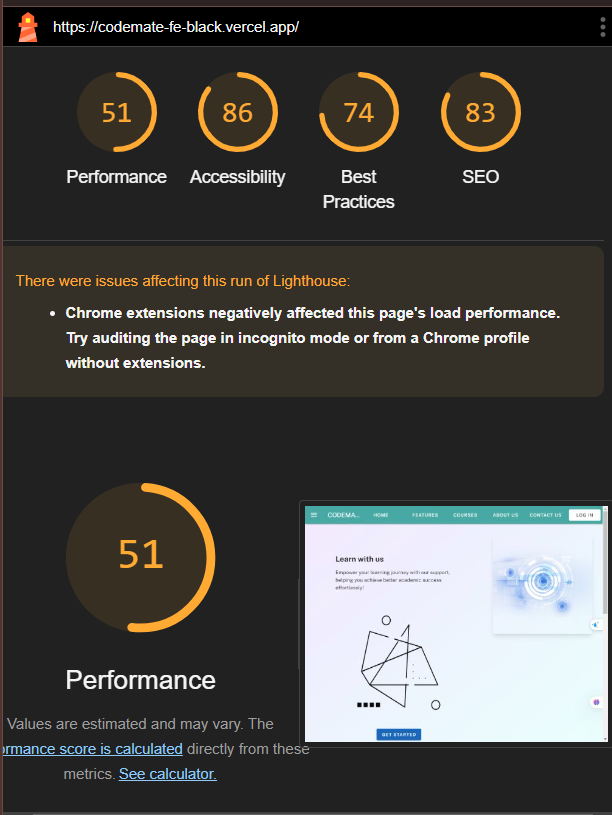
\includegraphics[width=\linewidth]{images/lighthouse_landing_space.png}
\end{minipage}
\hfill
\begin{minipage}{0.45\textwidth}
  \centering
  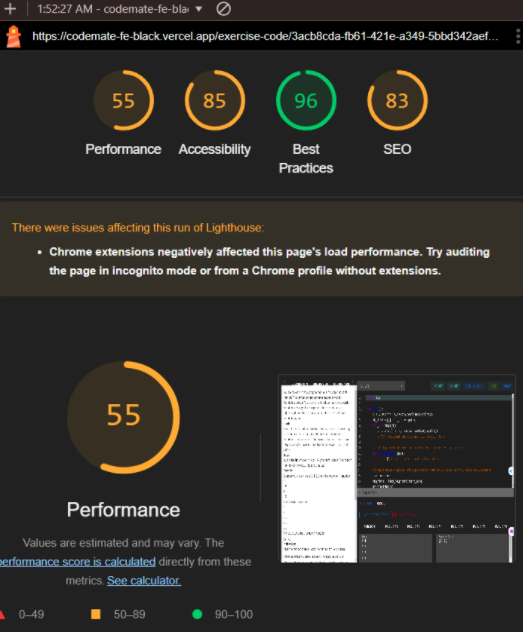
\includegraphics[width=\linewidth]{images/lighthouse_code.png}
\end{minipage}

\vspace{1em}

\begin{minipage}{0.45\textwidth}
  \centering
  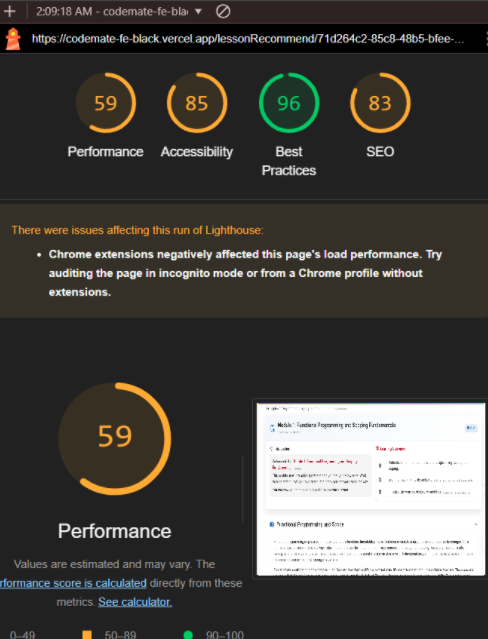
\includegraphics[width=\linewidth]{images/lighthouse_detail_module.png}
\end{minipage}
\hfill
\begin{minipage}{0.45\textwidth}
  \centering
  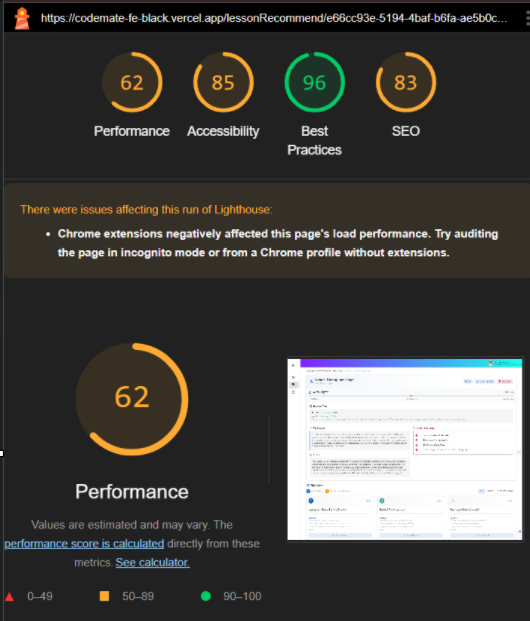
\includegraphics[width=\linewidth]{images/lighthouse_detail_lesson.png}
\end{minipage}

\vspace{1em}

\caption{Kết quả đánh giá một số trang bằng Lighthouse}
\end{figure}
